\section{Introduction}
\label{sec:intro}
Complex SQL queries may be written in several different ways and are difficult for beginners to get right. In courses that teach SQL queries, student SQL queries are often graded manually. The manual grading involves reading the student query manually comparing it to a correct query and/or executing the query on fixed datasets. Manually reading the query and comparing queries may be difficult and is also prone to errors while using grading using fixed datasets may miss errors in student queries. Let us consider an example where the correct query $Q$ is \\
\smalltt {\tabsql SELECT course.id, department.dept\_name \\\tabsql
FROM course LEFT OUTER JOIN \\\tabsql\tabsql
(SELECT * from department WHERE department.budget > 70000) d \\\tabsql
USING (dept\_name);}\\
A common mistake made by students is to write the following query $Q_s$ instead\\\tabsql
\smalltt{SELECT course.id, department.dept\_name \\\tabsql
FROM course LEFT OUTER JOIN department \\\tabsql
USING (dept\_name) WHERE department.budget > 70000;}

The student query looks sufficiently similar for a grader to miss the difference. The queries, however, are not equivalent since they give different results on departments with a budget less than 70000. The query $Q$ would output such courses with a NULL department name while $Q_s$ would not output such courses. Even using a fixed dataset may not be able to find the difference unless the dataset has a tuple where the department budget is less than 70000. Thus a fixed dataset may also miss such errors in grading. 

Even when the student query is incorrect, the grader is often expected to provide partial marks to the student query based on how close the student query is to being correct.  A naive approach of counting the number of datasets for which a query gives the correct answer may not be fair for partial marking since a small error may cause many or all test datasets to fail.  For example, if a student used a selection condition $a>10$ instead of $a<10$, most test datasets would fail. Conversely, a query with basic conceptual errors may still give the correct result on some datasets, especially ones where an empty answer is expected. 
Awarding partial marks manually is tedious and error-prone. Let us consider the following correct query provided by the instructor\\
\smalltt{\tabsql SELECT * FROM r INNER JOIN s ON (r.A=s.A) WHERE r.A>10}\\
and a student submitted the query \\
\smalltt{\tabsql SELECT * FROM r INNER JOIN s ON (r.A=s.B) WHERE s.A>10}\\
A grader manually evaluating the student query above may deduct marks for two errors - one for the join condition and another for the selection condition. However, if the join condition in the student query is fixed, the student query is equivalent to the given correct query since now r.A and s.A are equivalent in the student query. Hence only marks for one error should have been deducted. 

In a database course, it would also be helpful for the student to receive specific feedback as to where they went wrong and how their mistakes could have been corrected. This is very time-consuming for TAs and is rarely done well even for moderately sized classes.  With the growing popularity of online courses, where students expect instant feedback on the answers they submit there is an increasing need for automated and instantaneous feedback,   Manual grading does not scale for large online courses, and just showing datasets where the query gave a wrong result may not provide clear feedback to students. 

In our work on XData~\cite{xdata:vldbj15,xdata:icde15,xdata:comad}, we developed techniques to automatically grade student queries, given a set of correct queries. 
XData has two steps for grading student SQL queries as shown in Figure~\ref{fig:workflow}. The instructor first provides the question text and some correct queries. Based on the correct queries, XData generates multiple datasets that are tailored to catch different types of errors on the given queries. Since SQL queries may be written in several different ways, allowing instructors to specify multiple correct queries allows us to ensure more coverage of test cases. It also helps us get more query correct structures which is useful for our partial marking technique. The test data generation technique can also be used to test database queries and applications as described in \cite{xdata:vldbj15, xdata:icde18}. 

\begin{figure}
	\centering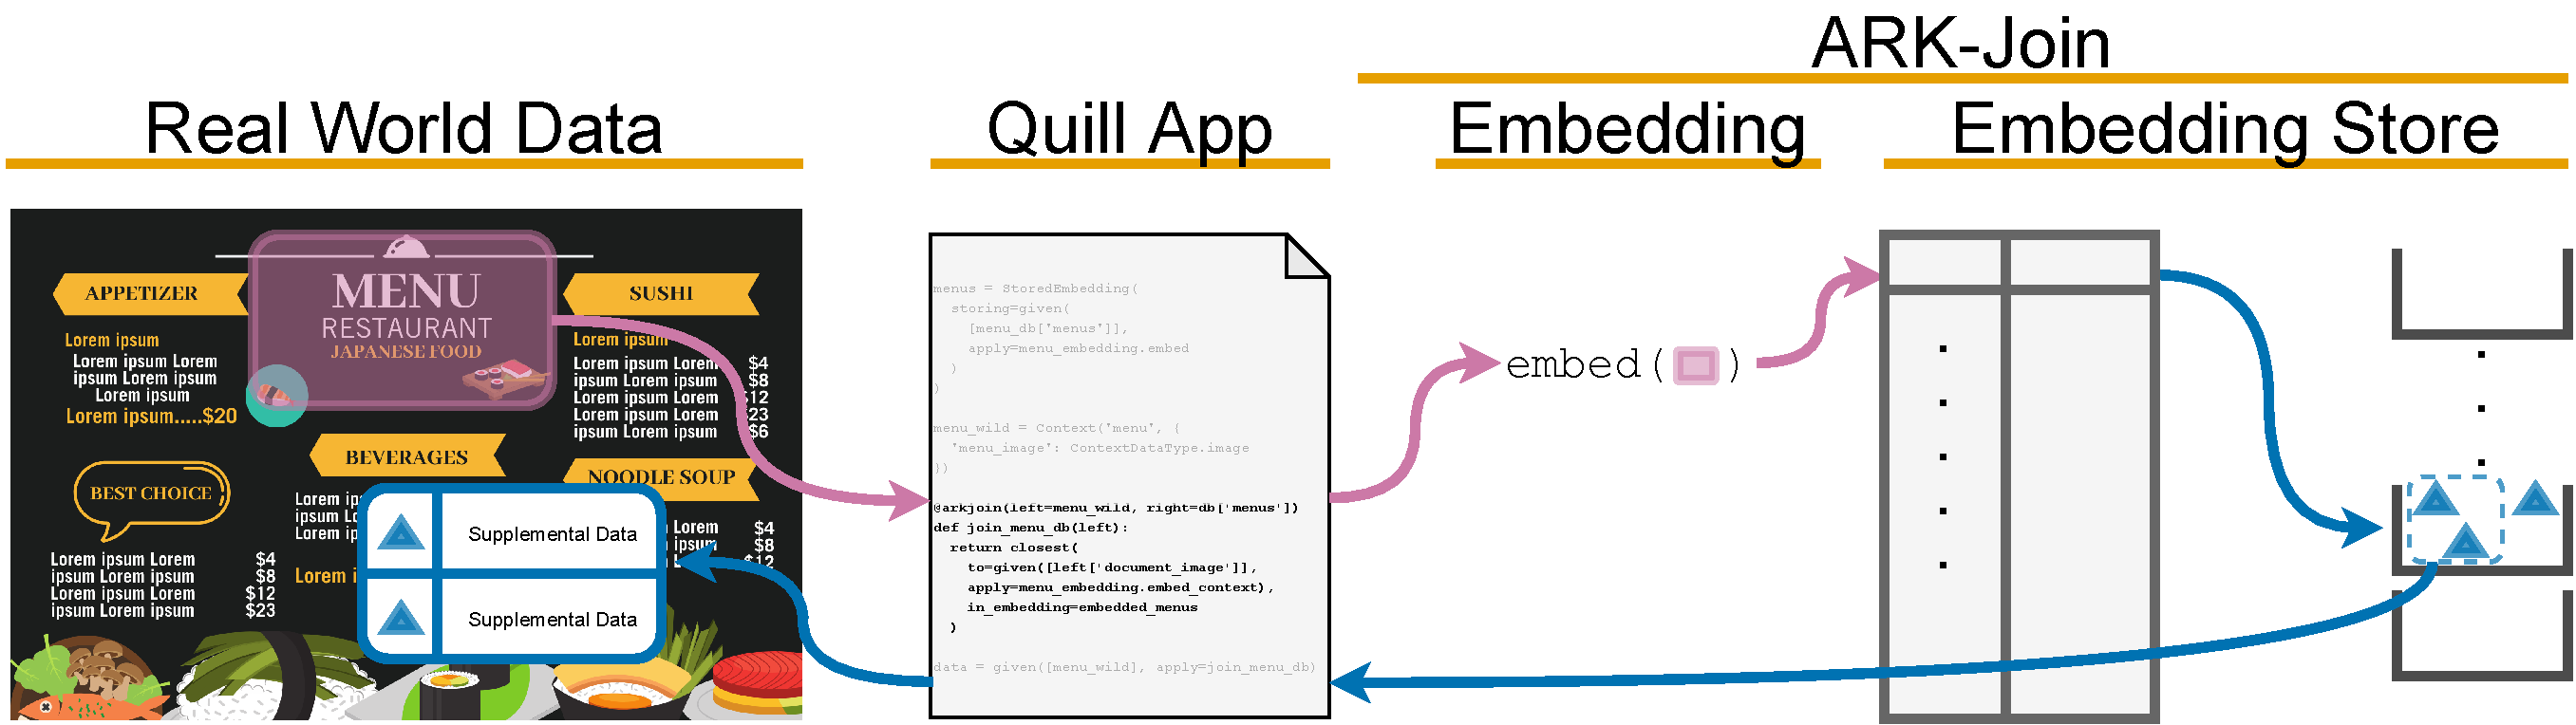
\includegraphics[width=0.67\textwidth,keepaspectratio=true]{workflow.pdf}
		\caption{Automated Grading Workflow}
		\label{fig:workflow}
\end{figure}


When evaluating a student query, the student query is run against the datasets generated by XData and the results are compared with the correct query. For correct student queries, the results generated by the student query and the instructor query would be the same across all generated datasets. Such queries would be awarded full marks. We note that techniques for checking query equivalence could potentially be used to check for equivalence of a student query to a correct query, but the state of the art for equivalence checking does not handle many SQL features such as null values, and has limitations in reasoning about equivalence with the given database constraints.  While there is a risk of labeling an incorrect query as correct using our approach, we have not found it to be an issue in practice.

For incorrect queries, XData compares the student query with the correct query using an edit-based technique and provides a score as well as the changes that need to be made in the student query to make it a correct query. Our approach scales to large class sizes and can grade student queries and provide feedback instantly. 

In this article, we first discuss, in Section~\ref{sec:intro}, techniques for automatically generating test data and how the test data generated can be used to check the correctness of SQL queries submitted by students. In Section~\ref{sec:edit}, we show how edit-based grading can be used to both award partial marks and provide individualized feedback for incorrect student queries. We share our experience of using the XData grading system in Section~\ref{sec:exp} and discuss related work in Section~\ref{sec:relwork}. We conclude the article in Section~\ref{sec:conclusion} and discuss some open challenges.  

